!! NOT fully written, I have to add some more info !!

The Engine for Likelihood-Free Inference (ELFI) \cite{1708.00707} is a Python software library dedicated to likelihood-free inference (LFI). ELFI models in a convenient manner all the fundamental components of a Probabilistic Model such as priors, simulators, summaries and distances. Furthermore, in the ELFI there are implemented a wide range of likelihood-free inference methods.

\subsubsection{Modelling}
\label{sec:modelling}

ELFI models the Probabilistic Model as Directed Acyclic Graph (DAG);
it implements this functionality based on the package NetworkX, which
is designed for creating general purpose graphs. Although not
restricted to that, in most cases the structure of a likelihood-free
model follows the pattern presented in figure \ref{fig:elfi-model};
there are edges that connect the \textit{prior} distributions to the
simulator, the simulator is connected to the summary statistics which
are connected to the distance, which is the output node. Samples can
be obtained from all nodes through sequential sampling. The nodes that
are defined as \textit{elfi.Prior}\footnote{The \textit{elfi.Prior}
  functionality is a wrapper around the scipy.stats package.} are
automatically considered as the parameters of interest and they are
the only nodes that should provide pdf evaluation, apart from
sampling. The function passed as argument in the \textit{elfi.Summary}
node can be any valid Python function with arguments the prior
variables.

\begin{figure}[!ht]
    \begin{center}
      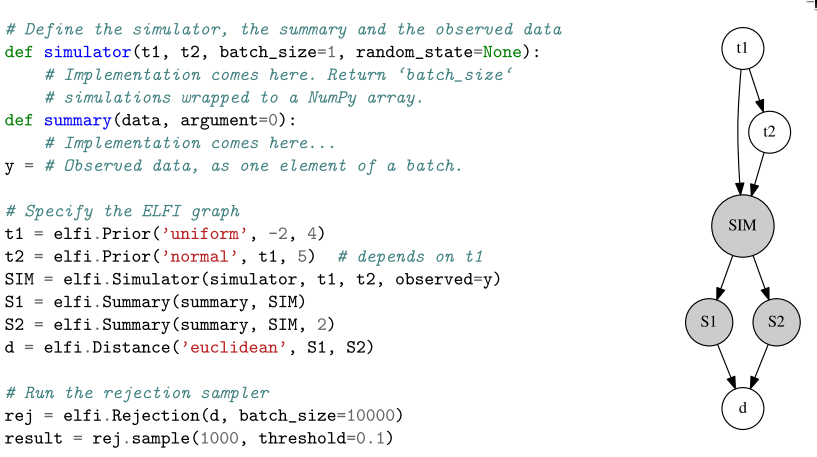
\includegraphics[width=0.8\textwidth]{./images/chapter2/elfi.png}
    \end{center}
    \caption{Image taken from \cite{1708.00707}}
    \label{fig:elfi-model}
\end{figure}


\subsubsection{Inference Methods}
\label{sec:inference-methods}

All Inference Methods that are implemented in ELFI, follow some common
guidelines; (a) their initialisation should by defined by passing the
output graph as the initial argument and afterwards come the rest
hyper-parameters of the method and (b) they must provide a basic
inference functionality, e.g. $<$\textit{method}$>$\textit{.sample()},
which returns a predefined \textit{elfi.Result} object containing the
obtained samples along with some other useful functionalities
(e.g. plotting the marginal posteriors).

A good collection of likelihood-free inference methods is implemented
so far, such as the \textit{ABC Rejection Sampler} and
\textit{Sequential Monte Carlo ABC Sampler}. A quite central method
implemented by ELFI is the \textit{Bayesian Optimisation for
  Likelihood-Free Inference (BOLFI)}, which is methodologically quite
close to the ROMC method we implement in the current dissertation.



